%++++++++++++++++++++++++++++++++++++++++
% Don't modify this section unless you know what you're doing!
\documentclass[letterpaper,12pt]{article}
\usepackage{tabularx} % extra features for tabular environment
\usepackage{amsmath}  % improve math presentation
\usepackage{graphicx} % takes care of graphic including machinery
\usepackage{amsfonts} 
\usepackage{float}
\usepackage{cite} % takes care of citations
\usepackage[utf8]{inputenc}
\usepackage{booktabs}
\usepackage[final]{hyperref} % adds hyper links inside the generated pdf file
\usepackage{listings}
\usepackage{xcolor}
\hypersetup{
	colorlinks=true,       % false: boxed links; true: colored links
	linkcolor=blue,        % color of internal links
	citecolor=blue,        % color of links to bibliography
	filecolor=magenta,     % color of file links
	urlcolor=blue         
}
\definecolor{lightgray}{rgb}{0.95, 0.95, 0.95}

\lstset{
  language=Python,
  basicstyle=\ttfamily,
  frame=single,
  backgroundcolor=\color{lightgray},
  numbers=left
}

%++++++++++++++++++++++++++++++++++++++++
\begin{document}
\begin{titlepage}
\begin{center}

\textsc{DATA ANALYSIS AND MACHINE LEARNING}\\
\textsc{FYS-STK4155}
\vspace{.3cm}

  {\LARGE
\textbf{Project 3}\par}
\vspace{3.5cm}
\hfill
\begin{minipage}{7cm}
Marco POZZOLI
\\
Lila CASSAN
\end{minipage}

\vfill

December 17, 2023

\end{center} 
\end{titlepage}


\newpage
\begin{abstract}
    The aim of this study was to find an efficient way of modeling the Forest Cover Types dataset, often used in Machine Learning. Three main algorithms were used: a Feed-Forward Neural Network , a Random Forest and XGboost.
    The XGboosting gave us the best accuracy (1.00) and was the fastest algorithm. The Random Forest gave us an efficient model but it was computationally expensive to find the most adequate number of tree. The Feed-Forward Neural Network (FFNN) gave us a satisfying result (0.90), but needs a tuning of much parameters and performs worse than the others algorithms. 
    
\end{abstract}


\newpage
\section{Introduction}
\par Forests play an important role in climate modeling due to their impact on carbon sequestration, oxygen release and biodiversity, and the use of machine learning algorithms helps to determine their structure and composition from data that can be collected more or less automatically, from ground observations or remote sensing data.
\par The Forest Cover Type dataset consists of ground observations made on forest plots. Our aim was to find the model fitting the best the dataset, in order to make accurate predictions. Modeling it allows us to develop an approach for other datasets to see what works best. Selecting this dataset also allows for working with a commonly used training dataset, which has been the subject of competitions, facilitating result comparisons.
\par In this study, we used three algorithms: Random Forest, Feed-Forward Neural Network, and XGboost whose parameters we adjusted.

\par This report is organized into three sections: Methods, Results, and Discussion. In the Methods section, We describe the techniques employed in our modeling of the Forest Cover Type dataset. The Results section presents the findings of our analysis, using different metrics. Finally, the Discussion section provides a comparative analysis of the two algorithms employed, as well as with previous studies.

\newpage
\section{Methods}

\subsection{Dataset}

For this project, we chose the "Forest Cover Type Dataset" \cite{forestcovertype}. It contains data from four areas of the Roosevelt National Forest in Colorado, tree observations in particular. 
All the observations refer to 30x30 meter sections of the forest. The dataset is quite big as it contains more than 500'000 measurements.\\
The original owners are Jock A. Blackard, Dr. Denis J. Dean, and Dr. Charles W. Anderson of the Remote Sensing and GIS Program at Colorado State University.\\
Our use for this dataset is to find which is the best model to predict what type of coverage a certain area has based on the other features.\\
The dataset contains features such as elevation, aspect, slope, horizontal distance to hydrology, vertical distance to hydrology, horizontal distance to roadways, horizontal distance to fire point, hillshade (at different times of the day), different types (4) of the wilderness area and of soil type (40).


\subsection{Metrics}
Here we introduce the metrics that we used to evaluate the quality and performance of the models.
\subsubsection{Accuracy}
The accuracy score is a simple metric given by the number of correct guesses ($t_i$) divided by the number of total guesses ($n$):
    \begin{equation}
        Accuracy = \frac{\sum_{i=1}^nI(t_i=y_i)}{n}
    \end{equation}
Where:
    \begin{equation}
        I = \begin{cases}
            1 \text{ if the condition is met}\\
            0 \text{ if the condition is not met}
            \end{cases}\,.
    \end{equation}
    
\subsubsection{ROC curve}
The ROC curve ($Receiver$ $Operating$ $Characteristic$ $Curve$) is a graph that represents the performance of a classification model at different thresholds.\\
This curve takes into account two parameters: TPR (True Positive Rate) on the y-axis and FPR (False Positive Rate) on the x-axis.\\
TPR is calculated on the amount of positive results among all positive samples available during the test. FPR is instead defined as how many incorrect positive results occur among all negative samples available during the test.
    \begin{equation}
        TPR = \frac{TP}{TP+FN}
    \end{equation}
    \begin{equation}
        FPR = \frac{FP}{FP+FN}
    \end{equation}
    \begin{figure}[H]
    \centering
    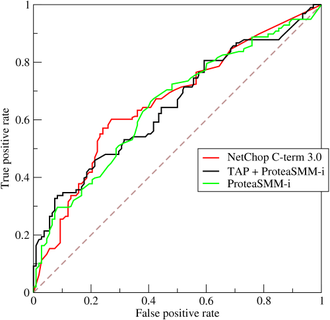
\includegraphics[width=5cm]{ROCex.png}
    \caption{\centering Example of a ROC curve. \cite{ROC_wifi}}
    \label{cross}
\end{figure}
\subsection{Feed-Forward Neural Network}
\par Describe the methods and algorithms
We use a Feed-Forward Neural Network, as described in \cite{proj2}. This architecture of Neural Networks corresponds to hidden layers with information going forward, and no feedback. The Neural Network allows us to obtain a model by adjusting weights in biases with a backpropagation pass, in an iterative process (see \cite{proj2} for further details).
\par In a first time, we tried to adjust our code for Project 2 for modelling the Forest Cover Type Dataset. The result diverged so we decided to use the library Tensorflow and the API Keras. After loading and reshaping our data, we create our neurons layers. We choose one hidden layer with 64 neurons, and an output layer consisting in 7 neurons. The number 7 correspond to the number of classes in the dataset, we have then a probability for each class. We choose an optimizer : ADAM with a learning rate $\gamma = 0.0001$. Then, we train the model, using our data. Finally, we can predict classes for given features, and compute metrics.

\begin{lstlisting}
model = keras.Sequential([
    layers.Dense(64, activation='relu',
    input_shape=[X_train.shape[1]]),
    layers.Dense(64, activation='relu'),
    layers.Dense(7, activation='softmax')
])

optimizer = Adam(learning_rate=10e-4)

model.compile(
    optimizer=optimizer,
    loss='sparse_categorical_crossentropy',
    metrics=['accuracy'],
)

\end{lstlisting}


\subsection{Decision Trees}
Decision trees are the key component and basic algorithm of random forests. The main idea behind them is finding features that are the most important in identifying the correct target and splitting the dataset along the values of the aforementioned features.\\
As the name suggests, decision trees are divided into $root$ $node$, $interior$ $nodes$, and the $final$ $leaf$ $nodes$/$leaves$. They're connected by $branches$.\\
A decision tree is grown by performing binary splitting, via an algorithm that tries splitting the dataset at different feature split points and tested with a cost function. The splitting is then performed on the resulting subtrees. This algorithm is $greedy$, as the optimal split is chosen at the current step, instead of anticipating future steps and selecting a split that could result in a more effective tree later on.\\
In constructing a classification tree, the Gini index or entropy are commonly employed to assess the effectiveness of a specific split. This is because these methods are more responsive to the purity of a node compared to the classification error rate.\\
The Gini index gives us an idea of how mixed the classes are after the split.\\
It's is defined as:
    \begin{equation}
        g = \sum_{k=1}^K p_{mk}(1-p_{mk})
    \end{equation}
Entropy measures how much information we would get by knowing the value of a feature.\\
It's is defined as:
    \begin{equation}
        s = -\sum_{k=1}^K p_{mk}\log{p_{mk}}
    \end{equation}
Where k = 1,...,K is the number of observations.\\
$p_{mk}$ represents the number of observations of a class $k$ in a region $R_m$ in a region $N_m$ observations. It's defined as:
    \begin{equation}
        p_{mk} = \frac{1}{N_m}\sum_{x_i \in R_,} I(y_i = k)
    \end{equation}
We can also visualize a tree as:
\begin{figure}[H]
    \centering
    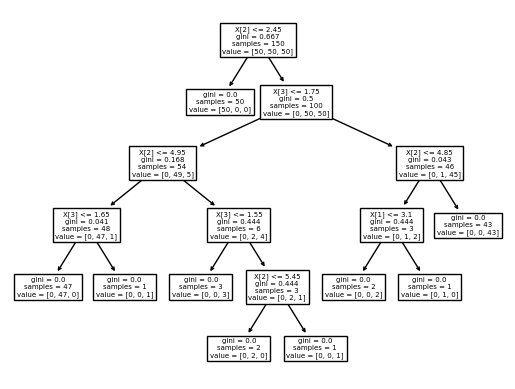
\includegraphics[width=11cm]{TREEex.png}
    \caption{\centering Example of a tree. \cite{lecnotes}}
    \label{cross}
\end{figure}

\subsection{Random Forest}
\par With a single decision tree, we often end up overfitting our training data, which implies a high variance. To reduce variance we introduce the $ensemble$ $methods$. One of these is $random$ $forests$.\\
In random forests, similarly to bagging, we build several decision trees on training samples obtained with bootstrapping. In the process of building the trees every time that a split is considered, a random sample of $m$ predictors is chosen as candidates for splitting from the full set of $p$ predictors. This way trees are different from each other and have a low correlation.\\
In classification problems, every tree votes for the most likely class, and the class with the most votes is taken as the final prediction of the model.\\
Random forests are effective on both classification and regression problems. Another important strength of random forests is that they are effective on large datasets with many variables, on the downside they're usually computationally intensive and may take a long time to use.\\
\par The code is fairly easy to implement thanks to Sci-kit Learn, a library that provides very useful tools for machine learning coding. After importing the libraries we load the data from our chosen dataset and split it into features (X) and target (Y), we then split it into training and testing. We scale it and we then create the random forest using sci-kit Learn, fit the data, and evaluate the model with the metrics that we previously introduced. The best parameters are found by performing a grid search.
\begin{figure}[H]
    \centering
    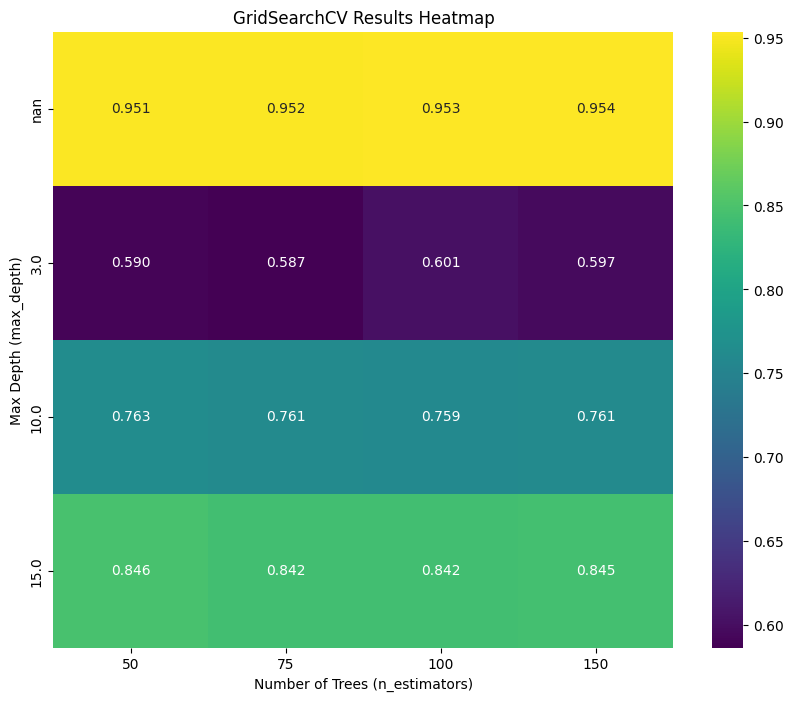
\includegraphics[width=11cm]{GSearch.png}
    \caption{\centering Results of the grid search for the optimal depth and number of trees.}
    \label{cross}
\end{figure}
The optimal parameters turn out to be depth = $none$ and n$\textunderscore$estimators = 150.

\subsection{XGBoost}
XGboost, which stands for $extreme$ $gradient$ $boosting$, is a gradient boosting library designed to make learning quicker and more precise. Since its invention and proposal, it has won several machine learning competitions.
We code it by using its library $xgboost$. With XGboost we also get a metric that gives us the importance of each feature in classifying data.
\begin{figure}[H]
    \centering
    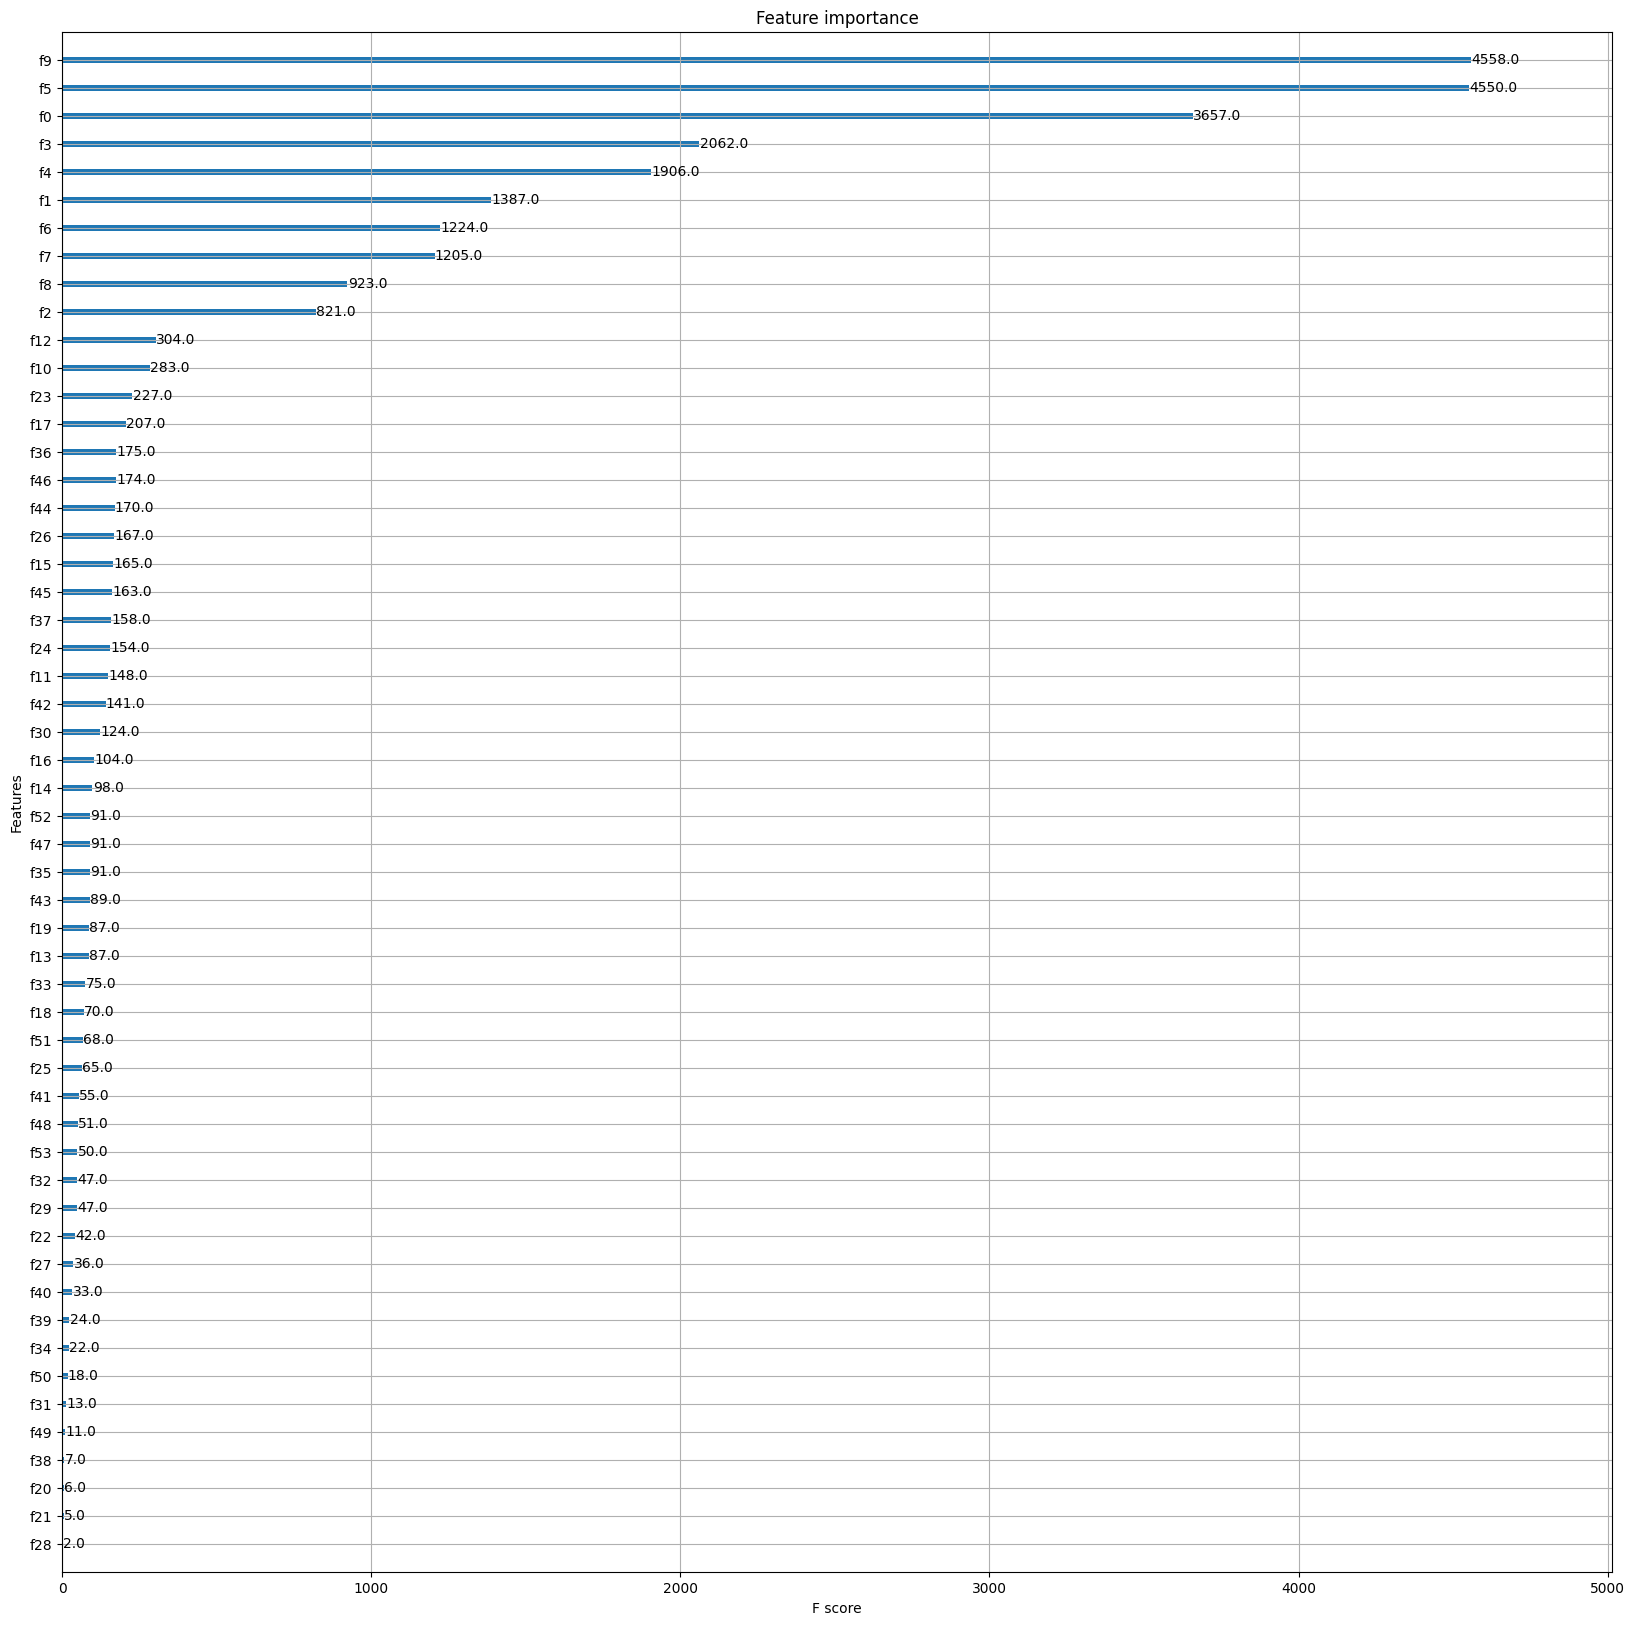
\includegraphics[width=13cm]{FeatImp.png}
    \caption{\centering Importance of each feature given by XGboost.}
    \label{cross}
\end{figure}
The most important features are by far horizontal distance to fire points (f9), horizontal distance to roadways (f5) and elevation (f0). The least important features for the prediction are, in general, soil types.
\newpage
\section{Results}

\subsection{Neural Network}
\par Using 30 epochs and one hidden layer, the ADAM optimizer with a learning rate $\gamma = 0.001$, the model accuracy increases really fast until approximately 10 epochs and then stabilizes. The model loss decreases significantly until 5 epochs and then stabilizes.
\begin{figure}[H]
    \centering
    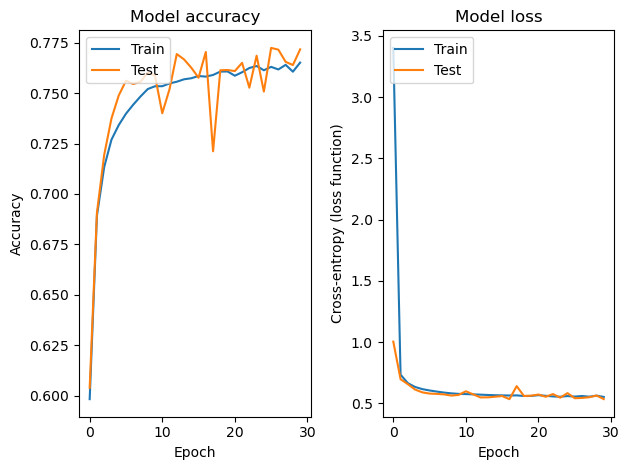
\includegraphics[width=11cm]{ModelAccuracyLost_FFNN.png}
    \caption{\centering Accuracy and Lost for a Feed Forward Neural Network with 1 hidden layer.}
    \label{FFNN_AccuLost}
\end{figure}

\par Running the following command:
\begin{lstlisting}
#fit the model
model_fitting = model.fit(
    X_train, y_train,
    validation_data = (X_test, y_test),
    verbose=1, epochs=30)  
\end{lstlisting}
took approximately 5 minutes and 30 seconds, even with a limited number of epochs (30). This limit does not allow us to try as many parameters combinations as we want.
\par After computing the ROC curves for our Feed-Forward Neural Network (Figure \ref{FFNN_ROC}, we obtain AUC (Area Under the Curve) values between 0.89 (class 2) and 1.00 (class 4) for each class against the other, which is satisfying \cite{MANDREKAR20101315}. The AUC value for micro-average of the ROC curve is 0.97, which means that our model can discriminate well between classes. The AUC value for micro-average of the ROC curve is 0.96, which means an adequate global performance of the model.
\begin{figure}[H]
    \centering
    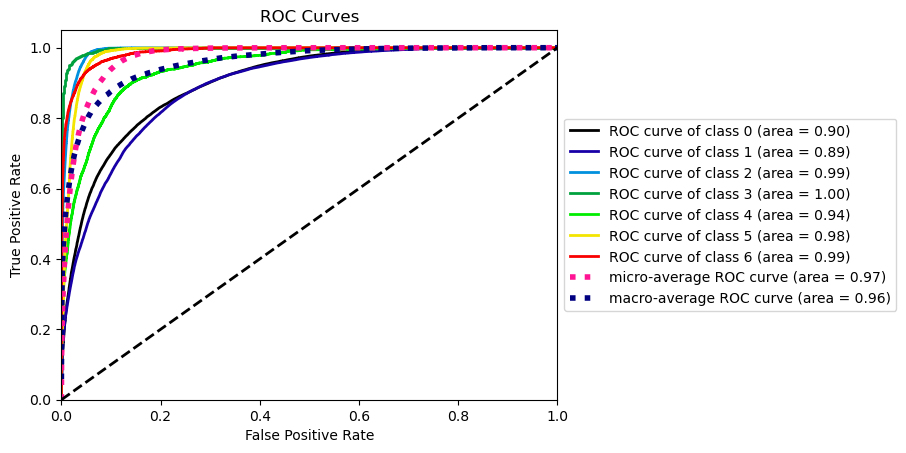
\includegraphics[width=11cm]{ROC_FFNN.png}
    \caption{\centering ROC Curve for a Feed Forward Neural Network with 2 hidden layers.}
    \label{FFNN_ROC}
\end{figure}
\par On the diagonal of the matrix, we want to have values near to 1. However, the label 1 was predicted with a probability of 0.74 where the true label was 4 and the correct label was only assigned with a probability 0.17. On the other side, the correct label was assigned with a probability of 0.89 for class 1. This means that our model can easily distinguish what can belong to class 1, but this class is predicted to too much inputs. 
\begin{figure}[H]
    \centering
    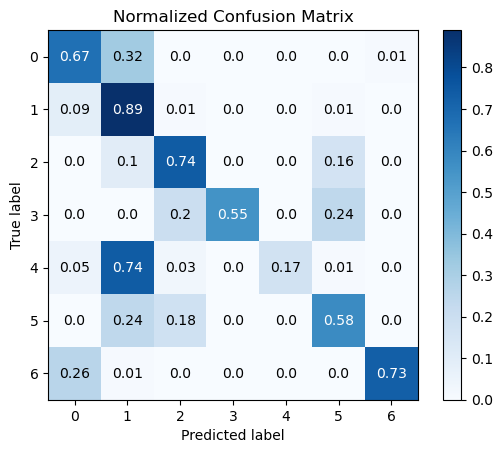
\includegraphics[width=11cm]{cm_FFNN.png}
    \caption{\centering Confusion Matrix a Feed Forward Neural Network with 2 hidden layers.}
    \label{FFNN_cm}
\end{figure}

We then ran the code multiple times to try to find the best parameters, and with 3 hidden layers of 120 neurons, the ADAM optimizer with a learning rate of $\gamma = 0.00001$ gave us a satisfying layer with an accuracy of 0.90 (Figure \ref{FFNN2_Acculost}), in 15 minutes. The number of epochs appears satisfying because the accuracy was in average still improving but with a small step.
\begin{figure}[H]
    \centering
    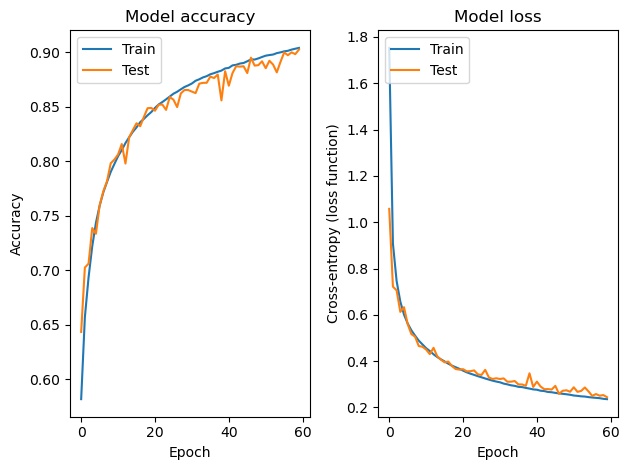
\includegraphics[width=11cm]{LossAccuracy9.png}
    \caption{\centering Accuracy and Lost for a Feed Forward Neural Network with 3 hidden layers of 120 neurons.}
    \label{FFNN2_Acculost}
\end{figure}

The area under the ROC curves was better also, and between 0.97 and 1 for all classes (Figure \ref{FFNN2_ROC})
\begin{figure}[H]
    \centering
    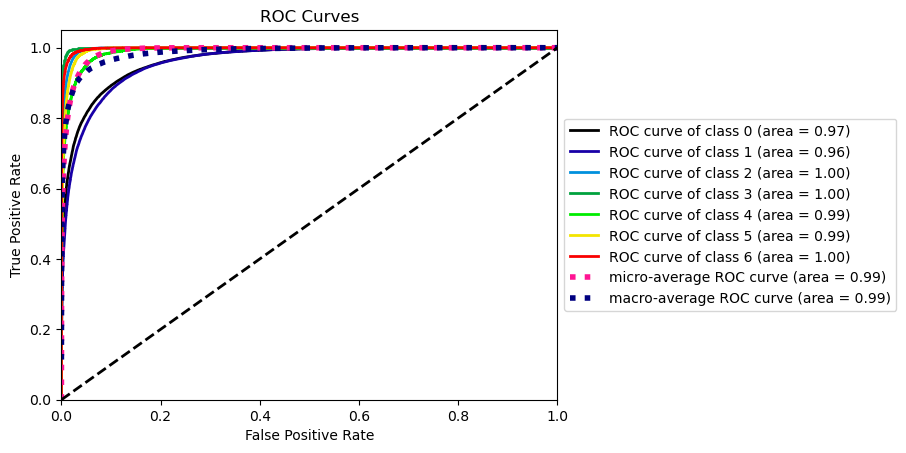
\includegraphics[width=11cm]{ROC9.png}
    \caption{\centering ROC curves for a Feed Forward Neural Network with 3 hidden layers of 120 neurons.}
    \label{FFNN2_ROC}
\end{figure}

The problem of confusion between classes 1 and 4 with our previous model was solved, and the value on the diagonal for class 4 is now better than 0.5, which means that our model is better than a random choice. However, it can still be improved because this value is much lower than for the other classes (0.67).
\begin{figure}[H]
    \centering
    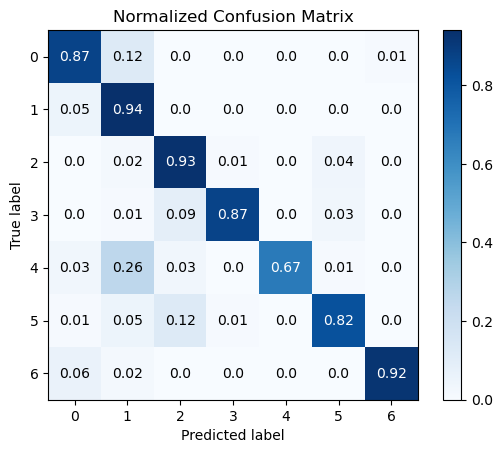
\includegraphics[width=11cm]{CM9.png}
    \caption{\centering Confusion matrix for a Feed Forward Neural Network with 3 hidden layers of 120 neurons.}
    \label{FFNN2_CM}
\end{figure}

\subsection{Random Forest}
Running the code section where the random forest is trained:
\begin{lstlisting}
#Random Forest fitting
#grid search's best params
best_params = grid_search.best_params_

optimized_rf = RandomForestClassifier(**best_params)

#we train the random forest model
optimized_rf.fit(X_train_scaled, y_train)
\end{lstlisting}
took around two hours. This is influenced by the size of the dataset and the computational power of the device on which the code is run.\\
After the data fitting, we take a look at the ROC curves.
\begin{figure}[H]
    \centering
    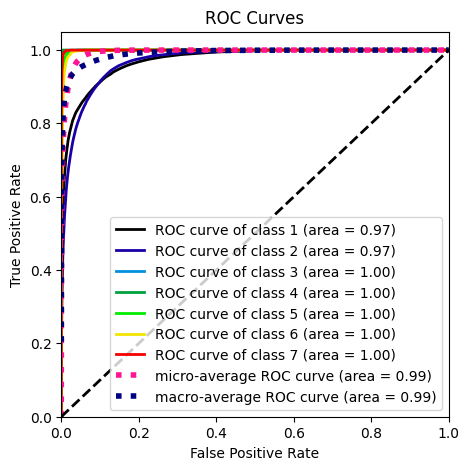
\includegraphics[width=7cm]{ROCRF.png}
    \caption{\centering ROC curves of our random forest.}
    \label{cross}
\end{figure}
The curves are very good, as almost every single one of them has an area of 1. Classes one and two have a slightly inferior area but are still very close to 1. Thus the random forest is a very good model for our classification problem and it can differentiate effectively.\\
We also take a look at the confusion matrix.
\begin{figure}[H]
    \centering
    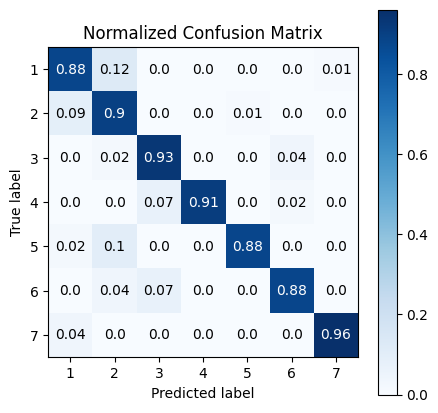
\includegraphics[width=7cm]{CMatrRF.png}
    \caption{\centering Confusion matrix of the random forest.}
    \label{cross}
\end{figure}
We can easily see how the Random forest sometimes fails to identify the right class. The predicted label is often mistaken for just one other true label, for example, the first class is sometimes mistaken almost only for the second.\\
The class that gets identified correctly more often is the seventh with an accuracy of 0.96, meanwhile, the hardest to predict correctly are the first, fifth, and sixth, with an equal accuracy of 0.88.

\subsection{XGboost}
The code for XGboost is:
\begin{lstlisting}
#XGboost training
xg_clf = xgb.XGBClassifier()
xg_clf.fit(X_train_scaled,y_train)
\end{lstlisting}
and it takes xxxx minutes to train.\\
We record an accuracy of 1.00, which makes the model perfect for our problem, as it predicts correctly every single time.\\
We now take a look at the ROC curve.
\begin{figure}[H]
    \centering
    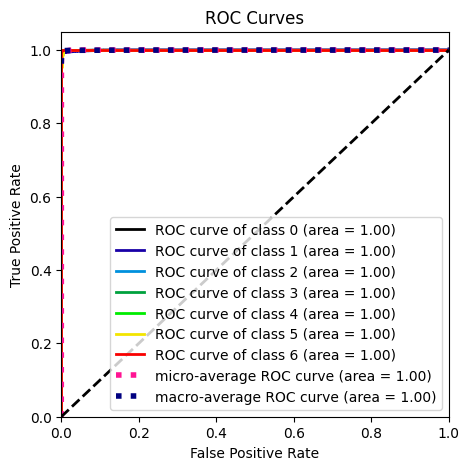
\includegraphics[width=7cm]{ROCXG.png}
    \caption{\centering ROC curves of XGboost.}
    \label{cross}
\end{figure}
All the curves are perfect: they all have an area of 1. This was expected, as we saw with accuracy that the XGboost model can perfectly predict the right cover type from the given features.\\
The confusion matrix is just as predictable:
\begin{figure}[H]
    \centering
    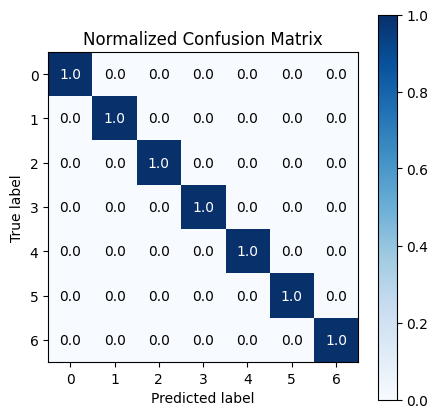
\includegraphics[width=7cm]{CMatrXG.png}
    \caption{\centering Confusion matrix of XGboost.}
    \label{cross}
\end{figure}
The matrix is a perfect diagonal.
\section{Discussion}
\subsection{Comparison}
We can now compare our results.
We start by comparing the accuracy of the three methods.
\begin{table}[ht]
\centering
\label{tab:ml_comparison}
\begin{tabular}{|l|c|}
\toprule
Algorithm & Accuracy \\ \midrule
Neural Network     & 0.904         \\
Random Forest     & 0.955         \\
XGboost     & 1.000         \\ \bottomrule
\end{tabular}
\caption{Accuracy for Neural Network, Random Forest and XGboost classifying the Forest Cover Type Dataset}
\end{table}\\
The best method is by far XGboosting (Table \ref{tab:ml_comparison}). It has perfect accuracy and never fails to identify the correct class. It's also very quick, taking only around 30 seconds to fit and predict.\\
The random forest is very accurate as well, even if it's not flawless, with an accuracy of 0.955.
Results obtained with Feed-Forward Neural Networks are not as accurate at the latters. However, it can still be improved by tuning different parameters (learning rate, number of epochs...), or by trying different algorithms for the optimizer.

\newpage
\section{Conclusion}
Our aim was to determine the best method for modelling the Forest Cover Type Dataset. Here, the XGBoosting give us the best results, and requires less time. It is possible to use different algorithms that can give us best results, but also to try different parameters to determine an efficient way to use Feed-Forward Neural Network.

\newpage
\section{Appendix}
Code: see \url{https://github.com/lilacandolle/Forest-Cover-Type}
\newpage
\bibliographystyle{plain}
\bibliography{References}

\end{document}
